
\documentclass[12pt]{article}


\usepackage{scicite}
\usepackage{hyperref}
\usepackage{graphicx}
\usepackage{caption} 
\usepackage{subfigure}
\usepackage{float}


\usepackage{times}


\topmargin 0.0cm
\oddsidemargin 0.2cm
\textwidth 16cm 
\textheight 21cm
\footskip 1.0cm



\newenvironment{sciabstract}{%
\begin{quote} \bf}
{\end{quote}}



\renewcommand\refname{References and Notes}


\newcounter{lastnote}
\newenvironment{scilastnote}{%
\setcounter{lastnote}{\value{enumiv}}%
\addtocounter{lastnote}{+1}%
\begin{list}%
{\arabic{lastnote}.}
{\setlength{\leftmargin}{.22in}}
{\setlength{\labelsep}{.5em}}}
{\end{list}}


% Include your paper's title here

\title{Deep speech} 


\author
{Vincent R\'ebiscoul, St\'ephane Pouget and Florent Gu\'epin}

% Include the date command, but leave its argument blank.

\date{}



%%%%%%%%%%%%%%%%% END OF PREAMBLE %%%%%%%%%%%%%%%%



\begin{document} 

% Double-space the manuscript.

\baselineskip24pt

% Make the title.

\maketitle 



% Place your abstract within the special {sciabstract} environment.

\begin{sciabstract}
  This document present our project in machine learning. We have implemented a voice recognition system. We use python3, Keras and Tensorflow.
\end{sciabstract}



\section*{Introduction}

We have implemented this artcile \cite{article} with python3, Keras and Tensorflow. The neuron network used is not common. So we created our own neuron network model.

\section*{Model}
We have seven layers of neuron. The three first layers are computed by :

\[ h_t^{(l)} = g(W^{(l)}h_t^{(l-1} + b^{(l)} \]

where $g(z) =$ min\{max $\{0,z\}, 20\}$

\begin{figure}[H]
\begin{center}
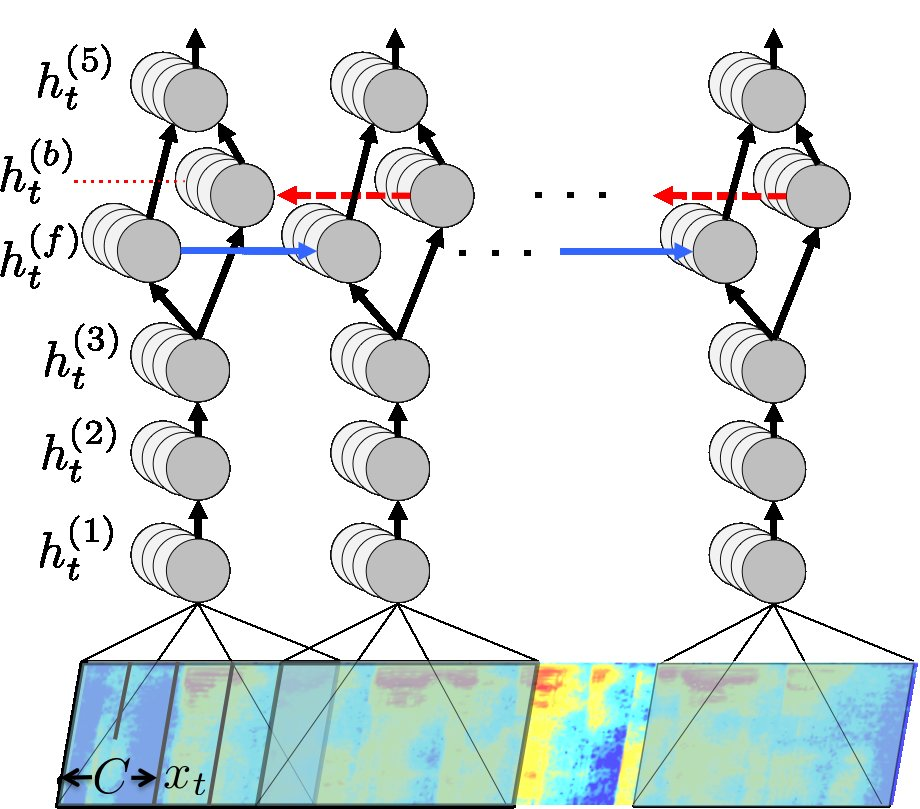
\includegraphics[scale=0.15]{images/photo.jpg}
\end{center}
\end{figure}

\section*{?}

\bibliography{scicite}

\bibliographystyle{Science}

\end{document}




















